\documentclass{article}
\usepackage{amsmath}
\usepackage{amssymb}
\usepackage{graphicx}
\usepackage{hyperref}
\usepackage[version=4]{mhchem}

\title{Example 11}
\date{}

\begin{document}
\maketitle

\(\triangle A B C\) is an isosceles triangle with \(A B=A C\) and \(\angle C A B=36^{\circ}\). Find the value of \(B C: A B\).

Solution: \(\frac{\sqrt{5}-1}{2}\).\\
\centering
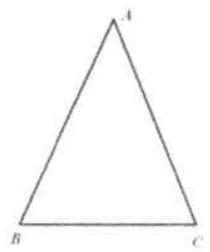
\includegraphics[width=\textwidth]{images/problem_image_1.jpg}


Let \(A B=A C=1\). Since \(\angle A=36^{\circ}, \angle B=\angle C=\frac{180^{\circ}-\angle A}{2}=72^{\circ}\).\\
Draw the angle bisector \(C D\) of \(\angle C\) where \(D\) is on \(A B\).\\
\(\angle B C D=\frac{1}{2} \angle A C B=36^{\circ}\).\\
So in \(\triangle B C D, \angle B C D=\angle B A C=36^{\circ}\) and \(\angle C B D=\angle A B C=72^{\circ}\).\\
Therefore, \(\triangle B C D \sim \triangle B A C\).\\
Let \(B C=x\). Since \(\angle B D C=\angle D B C=72^{\circ}, B C=C D\), so \(C D=x\).\\
Since \(\angle D C A=36^{\circ}=\angle A, C D=D A\).\\
Therefore \(A D=x\) and \(B D=1-x\).\\
Since \(\triangle B C D \sim \triangle B A C, \frac{B C}{B D}=\frac{A B}{B C}\).\\
\centering
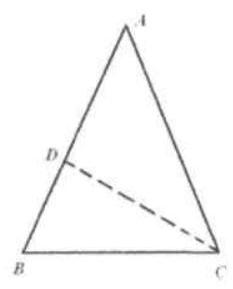
\includegraphics[width=\textwidth]{images/reasoning_image_1.jpg}

Therefore we have \(\frac{x}{1-x}=\frac{1}{x}\). Cross-multiplying gives us \(x^{2}+x-1=0\).\\
Solve for \(x\) : \(x=\frac{\sqrt{5}-1}{2}\). Hence \(\frac{B C}{A B}=\frac{x}{1}=\frac{\sqrt{5}-1}{2}\).\\

\end{document}
